\section{Frequency Calibration of Local Oscillators}\label{sec:calib}
The Q-Pix calibration requirements are described in detail in Section~\ref{sec:qpix_circuit}.
The important parameters which must be calibrated for each pixel are the charge per reset and the frequency of the local oscillator.
An aim of this work is to demonstrate an additional frequency calibration method using the minimal required connections between each digital node.

Any method of a frequency calibration must synchronize time measurements between all digital nodes within a tile and the aggregator.
There are several possible methods to achieve this, but ultimately the data that are recorded must be some time at the aggregator, $T_{a}$, and the time at any specific node, $T_{j}$.

%% distribute clock for calibration of time
A direct method is one where the aggregator distributes its own clock to all nodes in the tile.
This scenario removes the need for a calculation of the frequency of each node altogether since the clock of each node is already known from the aggregator.
This is the simplest case for timing calibration: remove all free running oscillators.

% cross-talk
A distributed clock network indeed removes ambiguity of the remote oscillator frequencies, but at the cost of hardware complexity.
Whether or not this design choice is preferred is entirely detector dependent, but likely increases in difficulty with the scale of the TPC.

We comment, however, that we ignore this scenario because it may altogether be unnecessary depending on future ASIC performance.
In the event that frequency calibrations of sufficient precision ($\bar{\delta f} \approx 1 \mathrm{ppm}$) are possible occur on free-running local oscillators future detectors would need only to acquire these ASICs and place them with minimal cost in terms of both time and money.

%% distribute trigger for calibration of time
Another simple scenario is one where the aggregator itself connects directly to all nodes within a tile via a single connection which can be used as a reference trigger.
This means that some trigger from the aggregator would issue directly into each node at the same time: $T_{a} = T_{n}$.
To calculate the frequency in this manner, the controller would issue two triggers from the aggregator with a known time separation, $T_{o} = T_{a2} - T_{a1}$.
The remote nodes would each record and send their timestamps back to the aggregator, where the time difference would be calculated as:

\begin{equation}
  T_{o} = T_{a2} - T_{a1} = T_{n2} - T_{n1}
\end{equation}

this is rewritten in terms of frequency as follows:
\begin{equation}
  f_{n} = \frac{T_{n2} - T_{n1}}{T_{o}}
\end{equation}

This calibration method, though extremely simple, introduces an additional connection to each ASIC between itself and the aggregator.
For a large scale system such as Q-Pix a single connection per ASIC introduces $\approx 60\times 10^{3}$ hardware points of failure per APA.

Both of these scenarios are valid implementations of a Q-Pix readout system.
In both of these scenarios, however, there is added complexity into the hardware design of the system in the form of additional routing where each route which represents a possible point of failure.

In a world of perfect hardware and costless routing in terms of both time and money these routing schemes would clearly be sufficient.
However, no hardware is perfect.
Therefore we introduce and discuss a calibration technique which relies on no additional routing and could be optionally implemented even in the above schemes in the event of a failure.
This calibration technique can be performed on any ASIC as long as it has a path back to the aggregator node, so can be used with any of the previously described routing schemes.

%% distribute packet for calibration of time
\subsection{A Minimal Connection Calibration Procedure}\label{sec:min_calib}
As stated previously, any frequency calibration records a reference time at the aggregator ($T_{a}$) and an event time ($T_{n}$) at an ASIC within a tile.
The time calibration procedure presented here requires only the minimal routing required in any Q-Pix readout system, where we assume time-dependent free-running local oscillators at each ASIC within the tile.

%% issue 1, then recv1
The calibration procedure begins at a time ($T_{0}$) where the aggregator sends a calibration packet.
Next, the packet propagates through the tile to some remote ASIC, $N_{j}$.
This ASIC receives the packet later at some time $T_{n1}$:

\begin{equation}
  T_{n1} = T_{o} + T_{f1}
\end{equation}


%% meas1 -> wait
Where $T_{f1}$ is the propagation time of the packet from the aggregator to the $N_{j}$ ASIC.
This remote ASIC then sends the packet with its time ($T_{n1}$) back to the aggregator.
The aggregator will wait some calibration time ($T_{cal}$) before issuing another calibration packet.
This wait period $\mathcal{O(10^{0-2})}$ can be long compared to the full transaction time to the $N_{j}$ ASIC $(\mathcal{O}(j*10^{-5})$).

%% issue 1
After the wait period, the aggregator will issue a second calibration packet to be sent to a remote ASIC at time:
\begin{equation}~\label{eq:calibration_wait_time}
  T_{1} = T_{cal} + T_{0}
\end{equation}

%% recv2 and meas2
Similarly to the first packet this packet will propagate to $N_{j}$ with some new time $T_{f2}$ where $N_{j}$ will record time $T_{n2}$:
\begin{equation}
  T_{n2} = T_{1} + T_{f2}
\end{equation}

Now, we define $\Delta T_{j}$ as the difference in the two time measurements from the two packets sent from the aggregator.
The time difference is related to the number of clocks that occurred between the two different measured values of the clock, $T_{n1}$ and $T_{n2}$.

\begin{equation}
  \Delta T_{j} = T_{n2} - T_{n1}
\end{equation}

We use the known relationships for $T_{n2}$ and $T_{n1}$ to obtain:
\begin{equation}
  \Delta T_{j} = (T_{1} + T_{f2}) - (T_{o} + T_{f1}) = (T_{1} - T_{0}) + (T_{f2} - T_{f1}) = T_{cal} + \Delta T_{f}
\end{equation}

Where we defined $\Delta T_{f}$ as the difference in forward propagation times from the packets sent from the aggregator at $T_{1}$ and $T_{0}$.

We arrive at the result which compares the measured time at the aggregator $T_{cal}$ and the time measured at each ASIC, $\Delta T_{j}$:
\begin{equation}
  \Delta T_{j} = T_{cal} + \Delta T_{f}
\end{equation}

A perfect reconstruction of the nodal frequency would follow if $\Delta T_{f} = 0$.
But it is sufficient to note that the wait period happens on the order of seconds, whereas $\Delta T_{f}$ is on the order of $\mu s$ or at least a six order of magnitude difference.
We then use $\Delta T_{f} \ll T_{cal}$ to obtain:
\begin{equation}
  \Delta T_{j} \approx T_{cal}
\end{equation}

We convert time into frequency with the difference of the timestamps measured and a known aggregator frequency ($f_{a}$):
\begin{equation}
   \frac{\Delta N_{j}}{f_{j}} = \frac{\Delta N_{a}}{f_{a}}
\end{equation}

or,
\begin{equation}~\label{eq:frequency_reconstruction}
   \boxed{f_{j} \simeq \frac{\Delta N_{j}}{\Delta N_{a}}f_{a}}
\end{equation}

Where $\Delta N_{j}$ and $\Delta N_{a}$ are the differences in the timestamps of the 32-bit clocks at the remote node and aggregator, respectively.


\subsubsection{Packet Transaction Time}
We next examine the approximation that $\Delta T_{f} \ll T_{cal}$ and consider its contribution to the error in the reconstruction of $T_{j}$ in Equation~\ref{eq:frequency_reconstruction}.
This analysis also provides a constraint on the duration of $T_{cal}$ (Equation~\ref{eq:calibration_wait_time}) to ensure an accurate measurement of each $T_{j}$ in a tile.
We begin by discussing how long it takes for a packet to traverse a tile.

The time it takes for each packet to be received by the next node is given in Equation~\ref{eq:t_packet}.
The value, $N_{bit}$, is the number of clock cycles used for the packet and is protocol-dependent.
Since the protocol is deterministic (Section~\ref{sec:endeavor}) for each packet, $N_{bits}$ is the same for each transaction on the path from the base node to the remote node.
As an example, the time it takes for a packet to go from the base node, $N_{1}$, to a remote node, $N_{3}$, via the path $1\rightarrow 2 \rightarrow 3$ is determined by:
%% packet transaction time
\begin{equation}~\label{eq:t_packetTransfer}
  T_{1\rightarrow 3} = T_{1\rightarrow 2} + T_{2\rightarrow 3} \approx \frac{N_{bits}}{f_{1}} + \frac{N_{bits}}{f_{2}} = N_{bits}(\frac{1}{f_{1}} + \frac{1}{f_{2}})
\end{equation}

Where, $f_{i}$, is the frequency of the clock at the sending node. 
The approximation in Equation~\ref{eq:t_packetTransfer} ignores variation less than a single clock cycle of the receiving digital node ($\approx 33~\unit{ns}$).
Therefore the time it takes for a packet for go from the base node to any remote node is proportional to $N_{bits}$ multiplied by the sum of the edges in the full adjacency matrix given by Equation~\ref{eq:adjacency_comp}.

We generalize Equation~\ref{eq:t_packetTransfer} to represent the time it takes a packet to go from the aggregator ($i = 0$) to any remote node, $N_{j}$:
\begin{equation}
  T_{f} = T_{0\rightarrow j} = N_{bits}\sum_{i=0}^{i=j-1}\frac{1}{f_{i}}
\end{equation}

We require that every calibration packet on the protocol uses the same number of clocks ($N_{bits}$ is the same for each identical Register Request, Section~\ref{sec:registers}).
$\Delta T_{f}$ becomes:
\begin{equation}
  \Delta T_{f} = N_{bits}\sum_{i=0}^{i=j-1}\frac{1}{\Delta f_{i}} = N_{bits} \sum_{i=0}^{i=j-1}\Delta T_{i}
\end{equation}

We recognize $\Delta T_{i}$ as the nominal time-dependent clock drift of the each local oscillator in the path between the base node to the remote-node.
We can provide an order of magnitude estimate for $\Delta T_{f}$ if we assume a (poor) $\approx 5\%$ drift in each of the remote clocks within the tile during a period of $T_{cal} \approx 1~\unit{s}$.
In this approximation we also assume that the mean of the periods of the nodes are the designed value ($\approx 33~\unit{ns}$) for which a 5\% error gives $\sigma_{T_{f}} \approx 15~\unit{ps}$.
If we further assume that all of the clocks drift systematically in the same direction (i.e., the mean drift doesn't cancel), then for 31 transactions (e.g., a 16$\times$16 tile broadcast) with 2000 clocks per transaction (Equation~\ref{eq:avg_packet}), we obtain for $\Delta T_{f}$:
\begin{equation}~\label{eq:calib_constraints}
  \Delta T_{f} \approx 2000 * 31 * 15\times 10^{-12} \approx 0.92~\unit{\mu s} 
\end{equation}

Equation~\ref{eq:calib_constraints} provides an estimation of the timing uncertainty introduced by the calibration scheme in a worst case 16$\times$16 tile scenario.
In the next section we introduce a prototype modular prototype board which was designed to test the stability of the communication protocol and the frequency calibration procedure presented here.

\section{The Q-Pix Digital Board}
\label{sec:qdb_prototype}
We describe the design of a modular digital back-end prototype board and discuss first results of the Q-Pix digital logic in an Field Programmable Gate Array (FPGA).
The results presented here constructed a tile 4$\times$4 array of Lattice iCE40UP5K-UWG30ITR FPGAs.
These FPGAs were chosen because of their small form factor, availability and pin out.
Each FPGA is programmed with the logic described in the previous sections based on the Q-Pix digital ASIC prototype.

The FPGAs are used to test the control logic, communication stability, buffer requirements, and calibration procedure which will be tested in the future Q-Pix digital prototype ASIC.
The most important quantity to be calibrated for the digital nodes is the frequency of the local oscillator.
The Q-Pix reconstruction for both time and z position are dependent on this parameter (see Chapter~\ref{chap:qpix}).

An example block diagram of the prototype board (QDB) is shown in Figure~\ref{fig:qdb_diagram}.
Each PCB connects 4 FPGAs in a 2$\times$2 array.
In the diagram shown, FPGA-A can connect to FPGA-B and FPGA-D, but not FPGA-C.
The external right angle bracket connectors are used to interconnect multiple tiles for a modular design.

\begin{figure}
\centering
\begin{subfigure}{.5\textwidth}
  \centering
  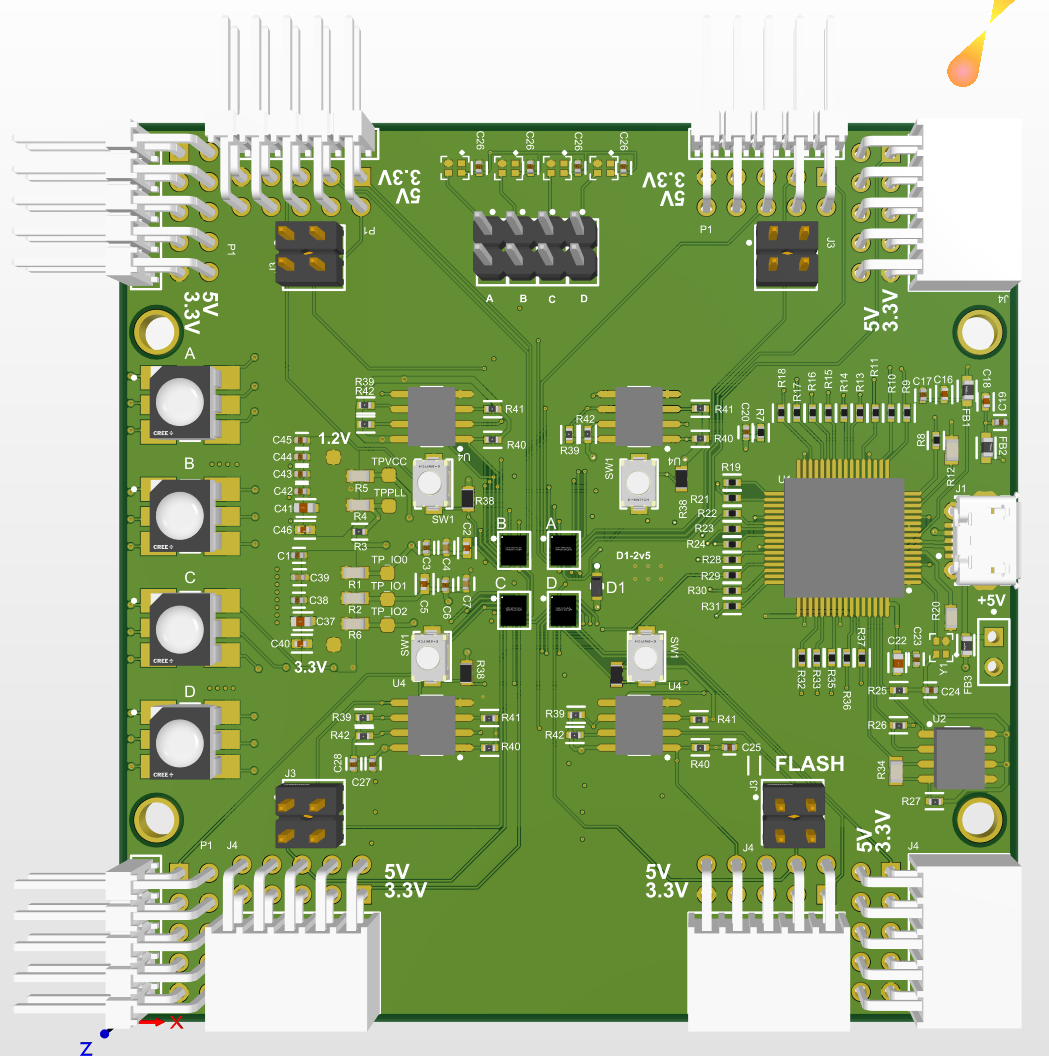
\includegraphics[width=\textwidth]{images/qdb_layout_altium.png}
  \caption{Q-Pix Digital Board (QDB) Design}
\end{subfigure}%
\begin{subfigure}{.5\textwidth}
  \centering
  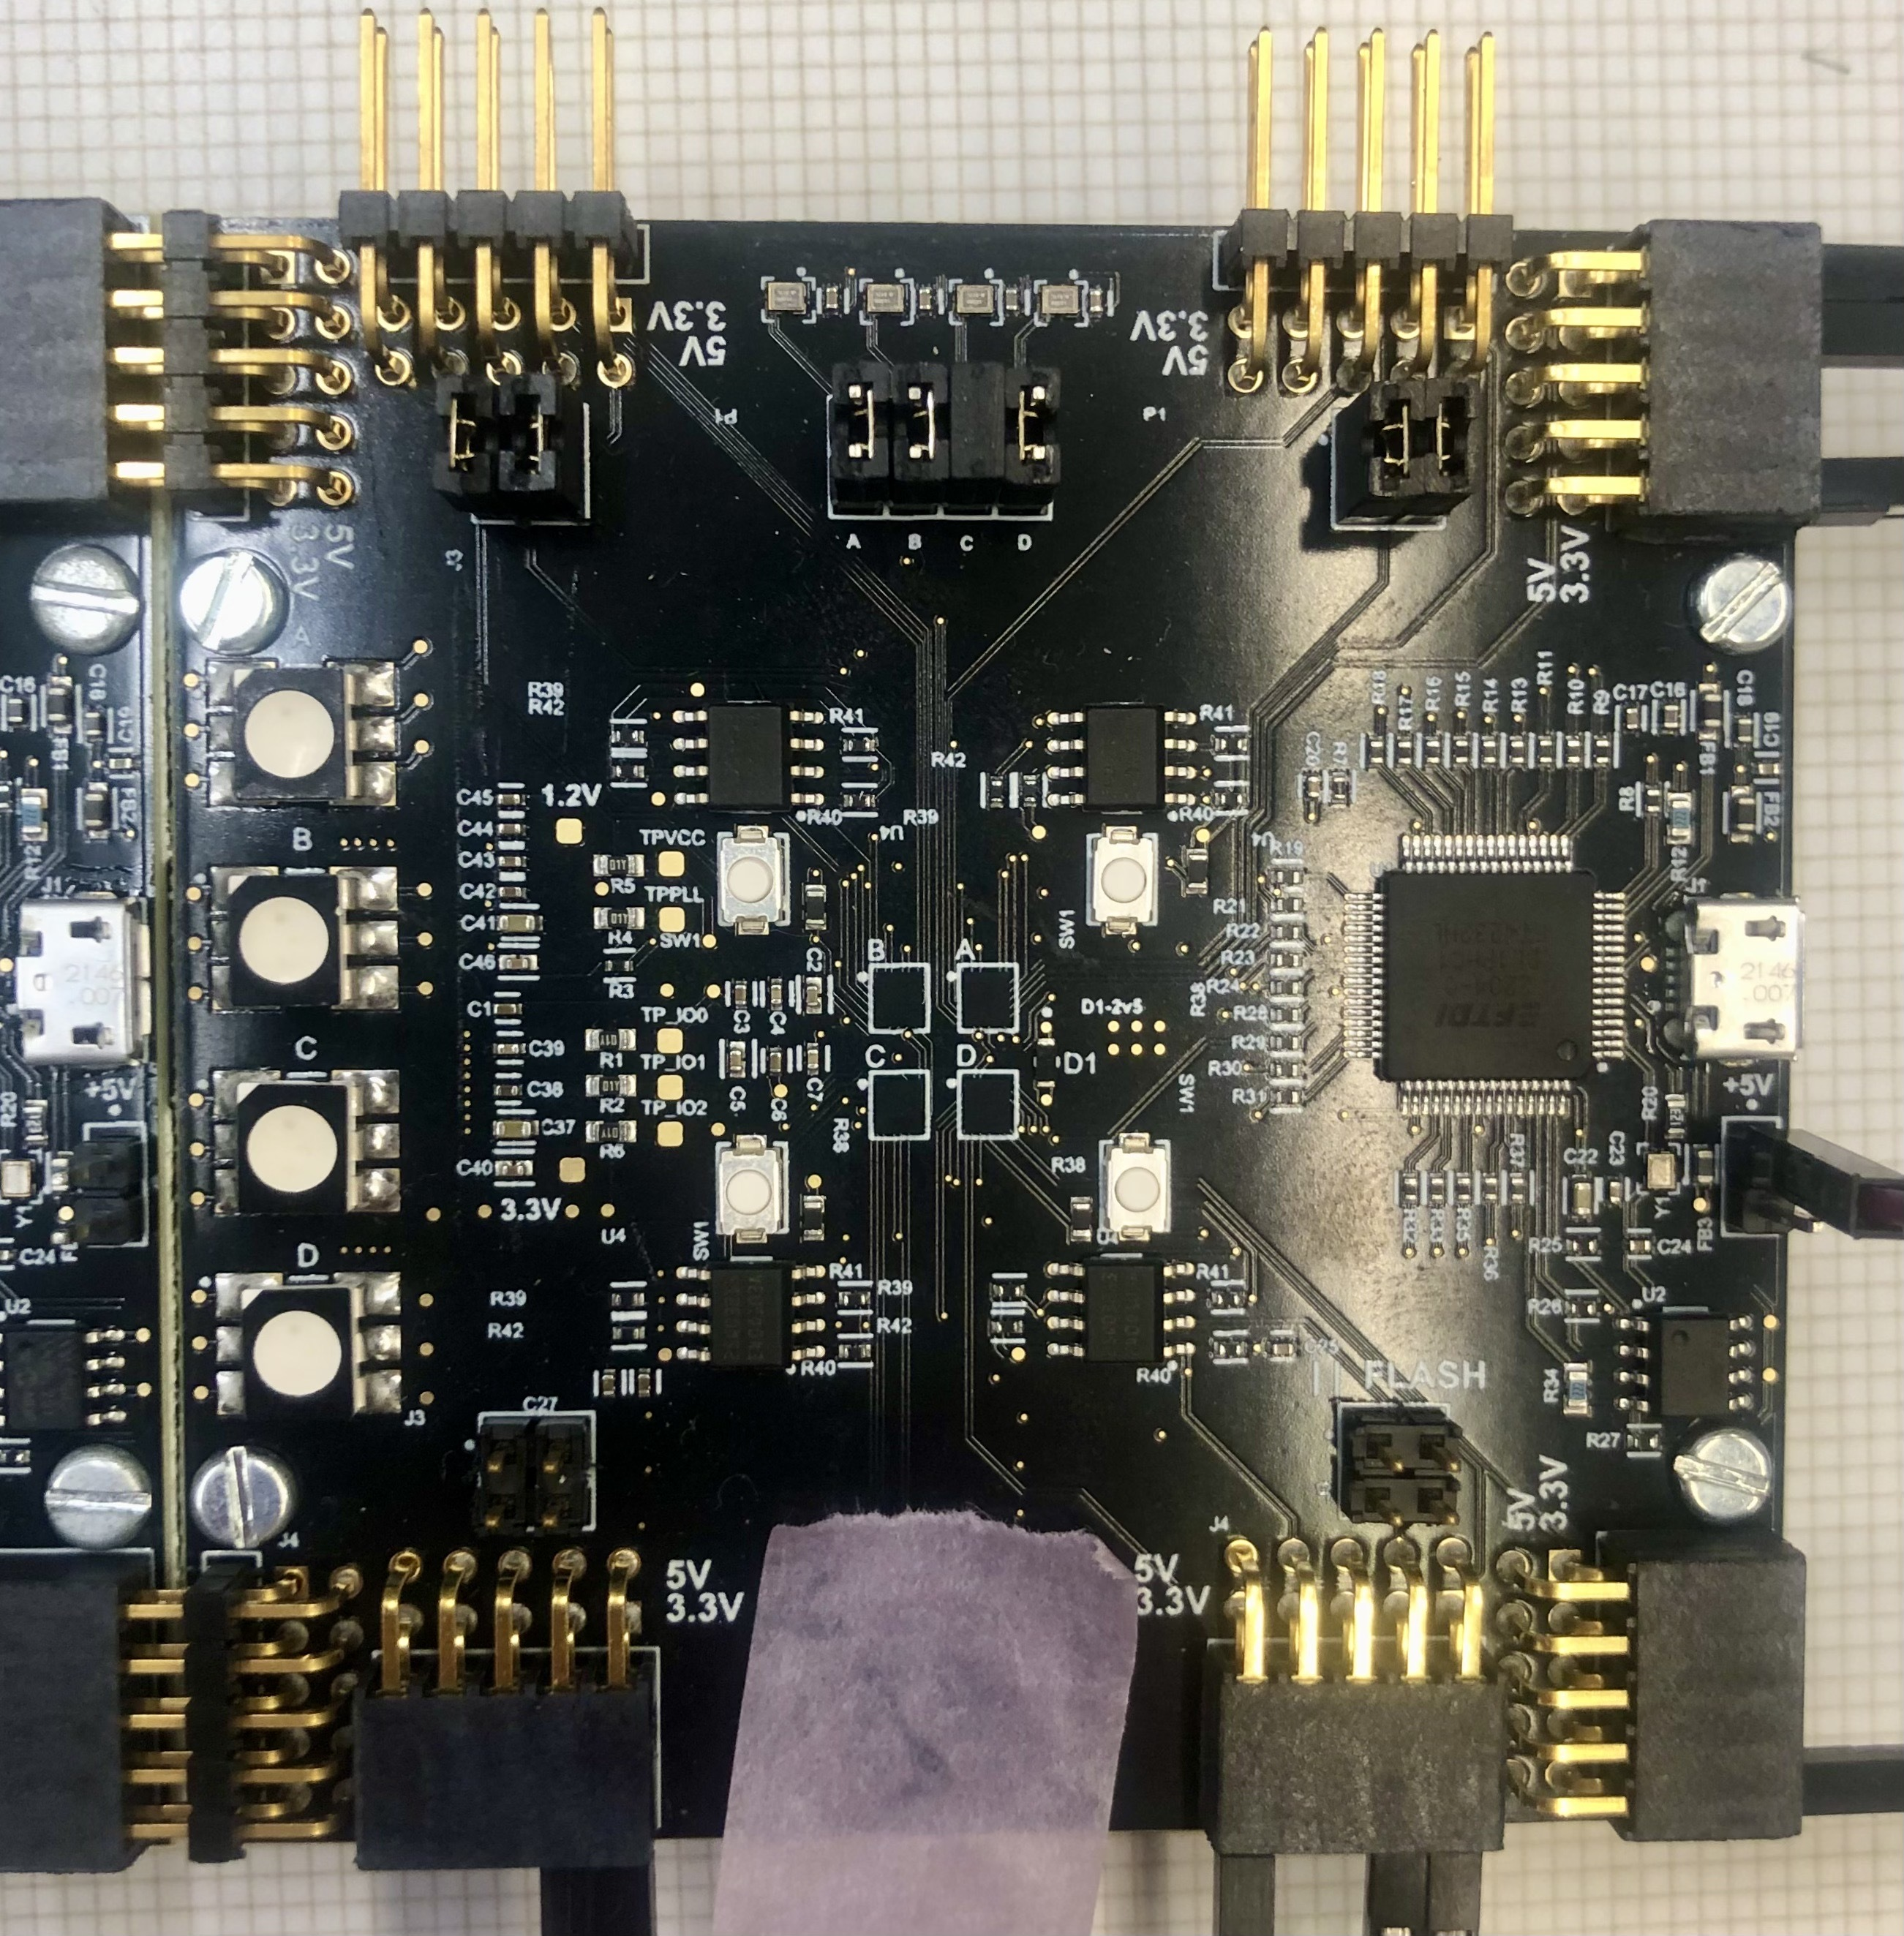
\includegraphics[width=\textwidth]{images/qdb_closeup.jpg}
  \caption{Q-Pix Digital Board (QDB) PCB}
\end{subfigure}
\caption{Layout of the Q-Pix Digital Board (QDB).}
\label{fig:qdb_diagram}
\end{figure}

Future implementations of the digital back-end for Q-Pix may, of course, use different oscillators.
However, these results are still beneficial as a proof of concept for the frequency calibration, as well as tests to the packet loss susceptibility.
Packet loss is a function of relative frequency drift between neighbor nodes.

Each iCE40 FPGA is uses an 12~\unit{MHz} external oscillator~\citep{ecs1612mv}, which is then connected to a phase-locked loop (PLL).
The PLL uses a multiply by five and divide by three circuit to achieve the desired 30~\unit{MHz} average frequency.
The PLL is a special IP for the iCE40UP5k FPGA's~\citep{latticeice40up}.

FPGA's are labeled A through D on each QDB, beginning in the "top-right" of the board and proceeding counter-clock wise, as shown in Figure~\ref{fig:qdb_diagram}.
Each FPGA has access to two right-angle connectors, which allow the QDBs to be inter-connected into a larger tile as shown in Figure~\ref{fig:qdb_test_setup}.
The numerical location (x,y) of each FPGA corresponds to number of transactions "left" or "right" (x), and "up" or "down" (y) from the aggregator as viewing in Figure~\ref{fig:qdb_diagram}.

We use the Zybo-Z7 prototype board from digilent as the aggregator node.
Communication to and from the board uses a custom software interface that allows data communication between the Zybo and a PC.
This DAQ is nearly identical to the procedure used in the SAQ experiment in Chapter~\ref{chap:saq}.

\begin{figure}[]
\centering
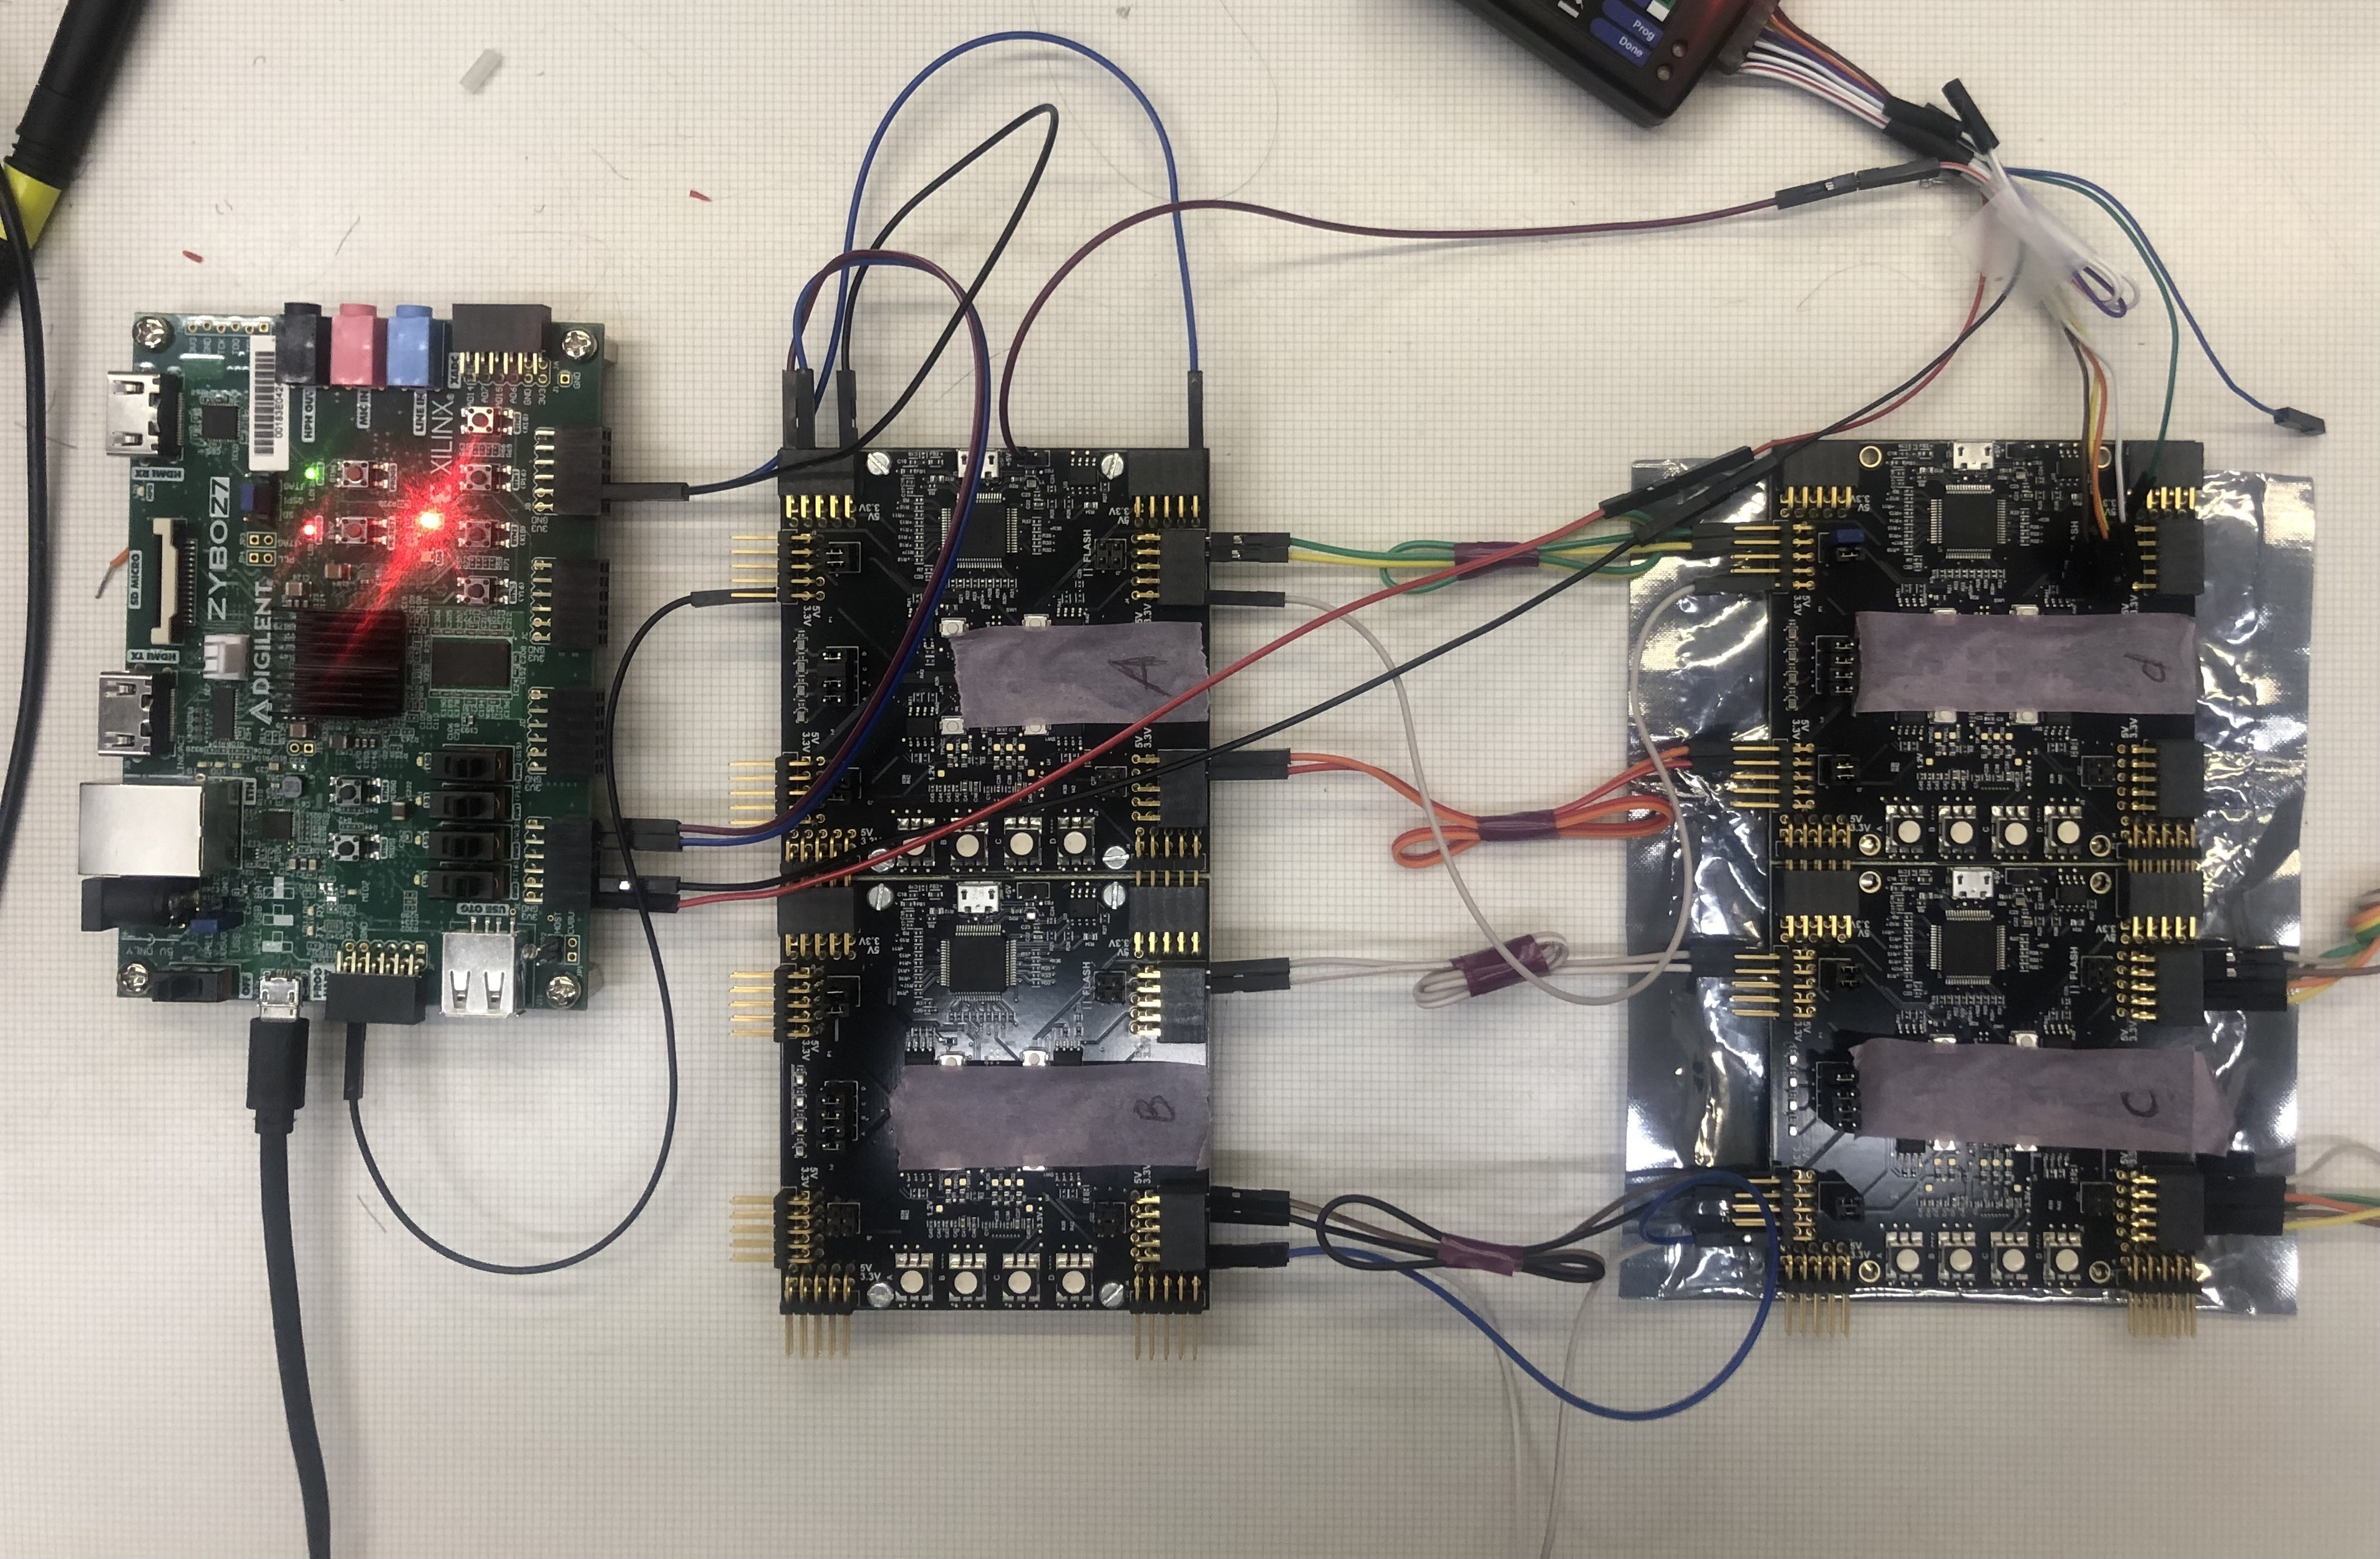
\includegraphics[width=0.8\textwidth]{./images/qdb_frequency_test_setup.jpg}
\caption{Layout of a Zybo-Z7 aggregator node connected to a single FPGA in an interconnected 2$\times$2 QDB Tile.
The total amount of interconnected FPGAs for the tile size is 4$\times$4.
The FPGA that connects to the Zybo is FPGA-A as shown in Figure~\ref{fig:qdb_diagram} on Board-A.
Not shown is the Ethernet connection from the Zybo back to the controlling PC.
Some QDB boards are connected via jumper wires to allow easier programming of the FPGAs and for probing pins.
}
\label{fig:qdb_test_setup}
\end{figure}

One of the main objectives of the prototype boards is to verify the communication protocol (Section~\ref{sec:comms}).
An example of a broadcast transaction between the Zybo and two FPGAs on a single QDB is shown in Figure~\ref{fig:example_broadcast}.
The transaction depicted is a broadcast register write, written to the command register (Table~\ref{table:node_registers}).
From left to right in image A, the packets follow this pattern:

\begin{enumerate}
  \item Zybo sends broadcast register write (hard interrogation)
  \item FPGA-A forwards and responds to broadcast and responds
  \item FPGA-B responds to broadcast 
  \item FPGA-A routes the remote packet to the Zybo
\end{enumerate}

\begin{figure}
\centering
\begin{subfigure}{0.475\textwidth}
  \centering
  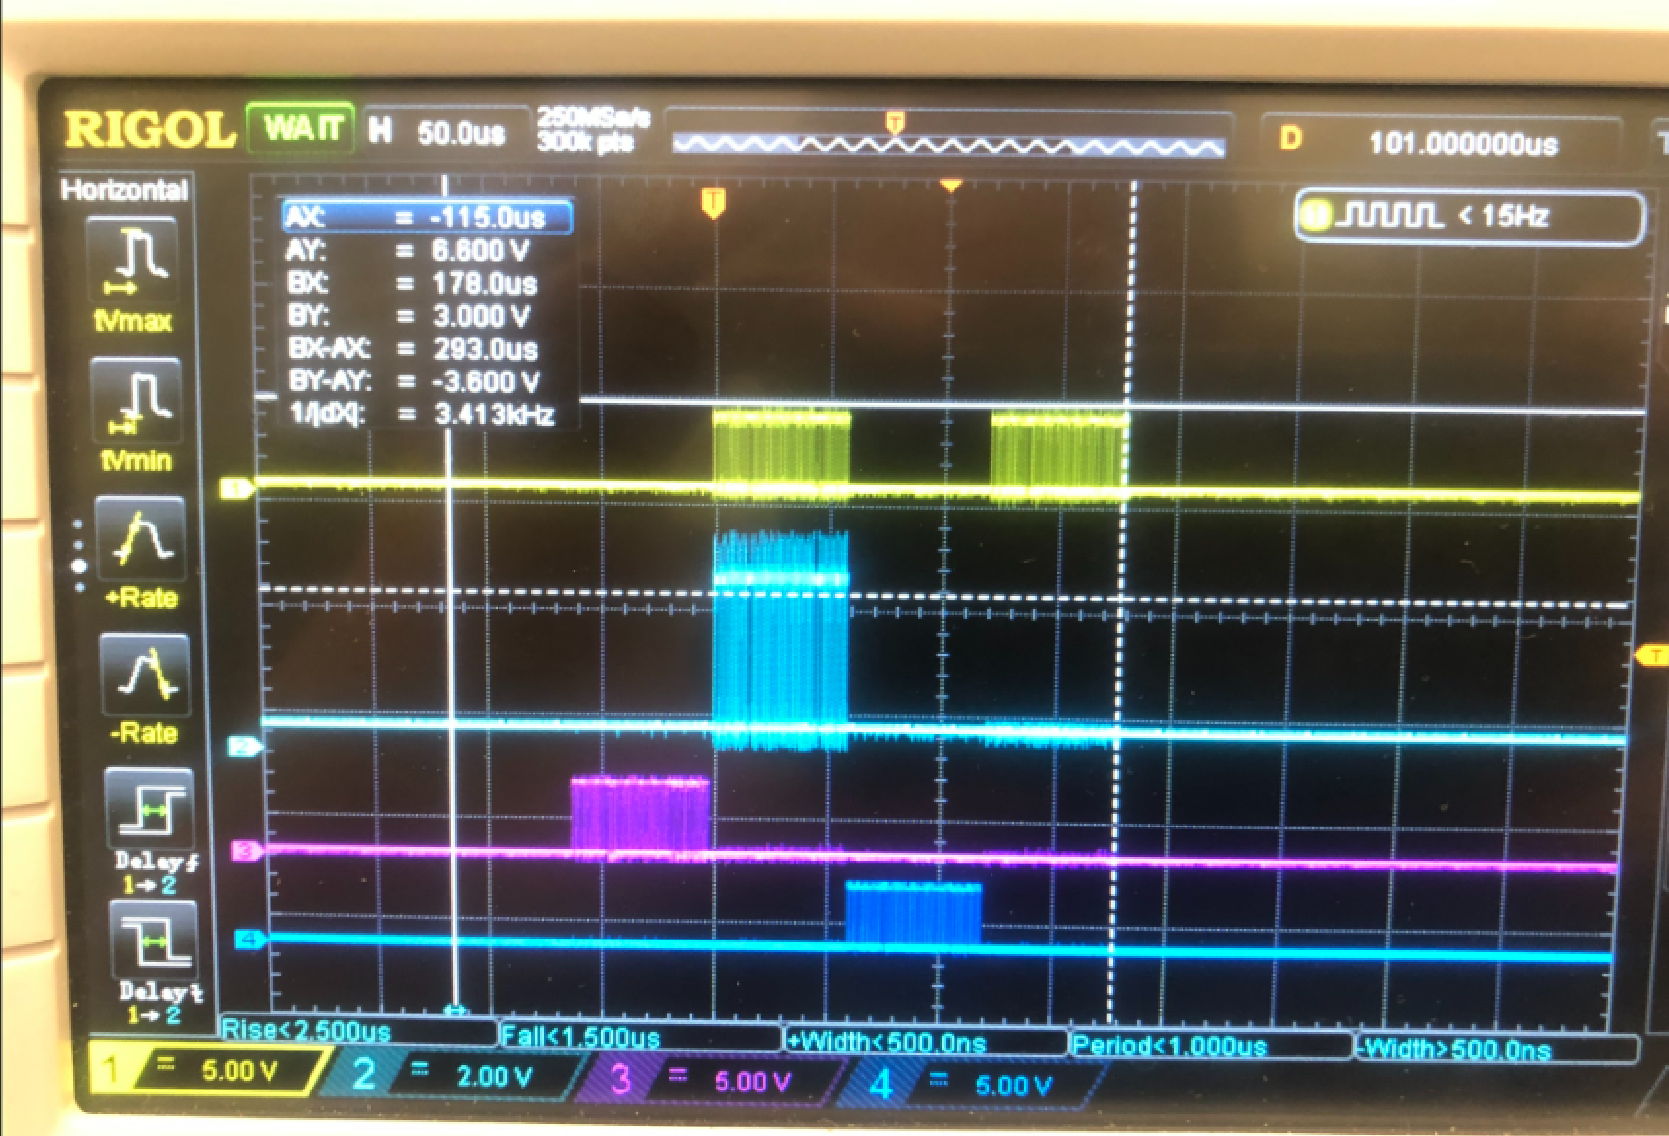
\includegraphics[width=\textwidth]{images/qdb_example_packet_waveform.png}
  \caption{Example of a Hard interrogation.}
\end{subfigure}%
\begin{subfigure}{0.475\textwidth}
  \centering
  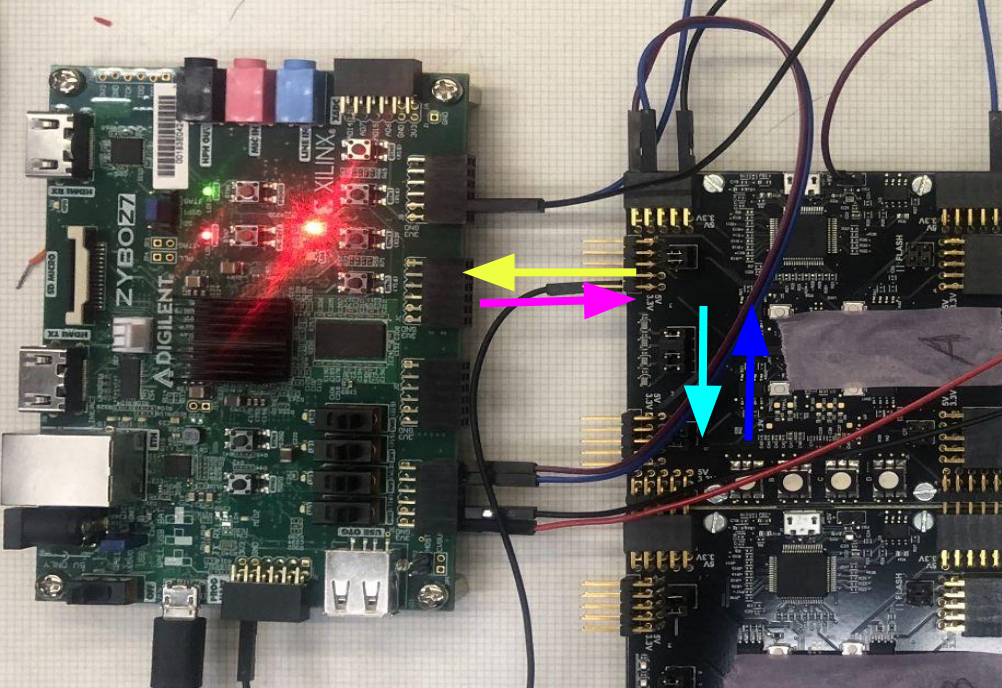
\includegraphics[width=\textwidth]{images/qdb_example_packet_waveform_diagram.png}
  \caption{Communication Route on Prototype}
\end{subfigure}
\caption{Timescale is 50 $\unit{\mu s}$.
An example of a hard interrogation with two connected FPGAs is shown.
The first incoming packet is the broadcast (register write to command register) from the Zybo board.
The FPGA (0,0) responds and sends the broadcast.
The bottom waveform is FPGA (1,0) responding to the request sent from (0,0).
The right image shows the direction of the packets as viewed on the QDB tile.
}
\label{fig:example_broadcast}
\end{figure}

\section{Prototype Frequency Calibration Results}
\label{sec:freq_calib_results}
We describe here the methods of measuring a stable oscillator frequency for the prototype PCB based on the frequency calibration scheme developed in Section~\ref{sec:calib}.

The interrogation procedure involves using a hard interrogation on the FPGA to ensure that each FPGA responds with an Event End packet (packets defined in Section~\ref{sec:local_data_packet}).
The Zybo records the time that it sends the interrogation time and collects 16 response packets from each FPGA.
We test the effects of the calibration rate ($T_{cal}$ in Equation~\ref{eq:calibration_wait_time}) by performing two sets of interrogation rates at 0.1~\unit{Hz} and 4~\unit{Hz}, which we refer to as the "slow" and "fast" interrogation rates.
The slow (0.1~\unit{Hz}) frequency test is the expected lower limit of reset data to be acquired from radiogenic and noise contributions alone (Section~\ref{sec:radiogenic_calib}).
The fast (4~\unit{Hz}) test allows only 250~\unit{ms} for a tile readout and is much faster than any interrogation requirement for use in a DUNE-FD APA ($\simeq$~1~\unit{Hz} for beam spills). 

\begin{figure}[]
\centering
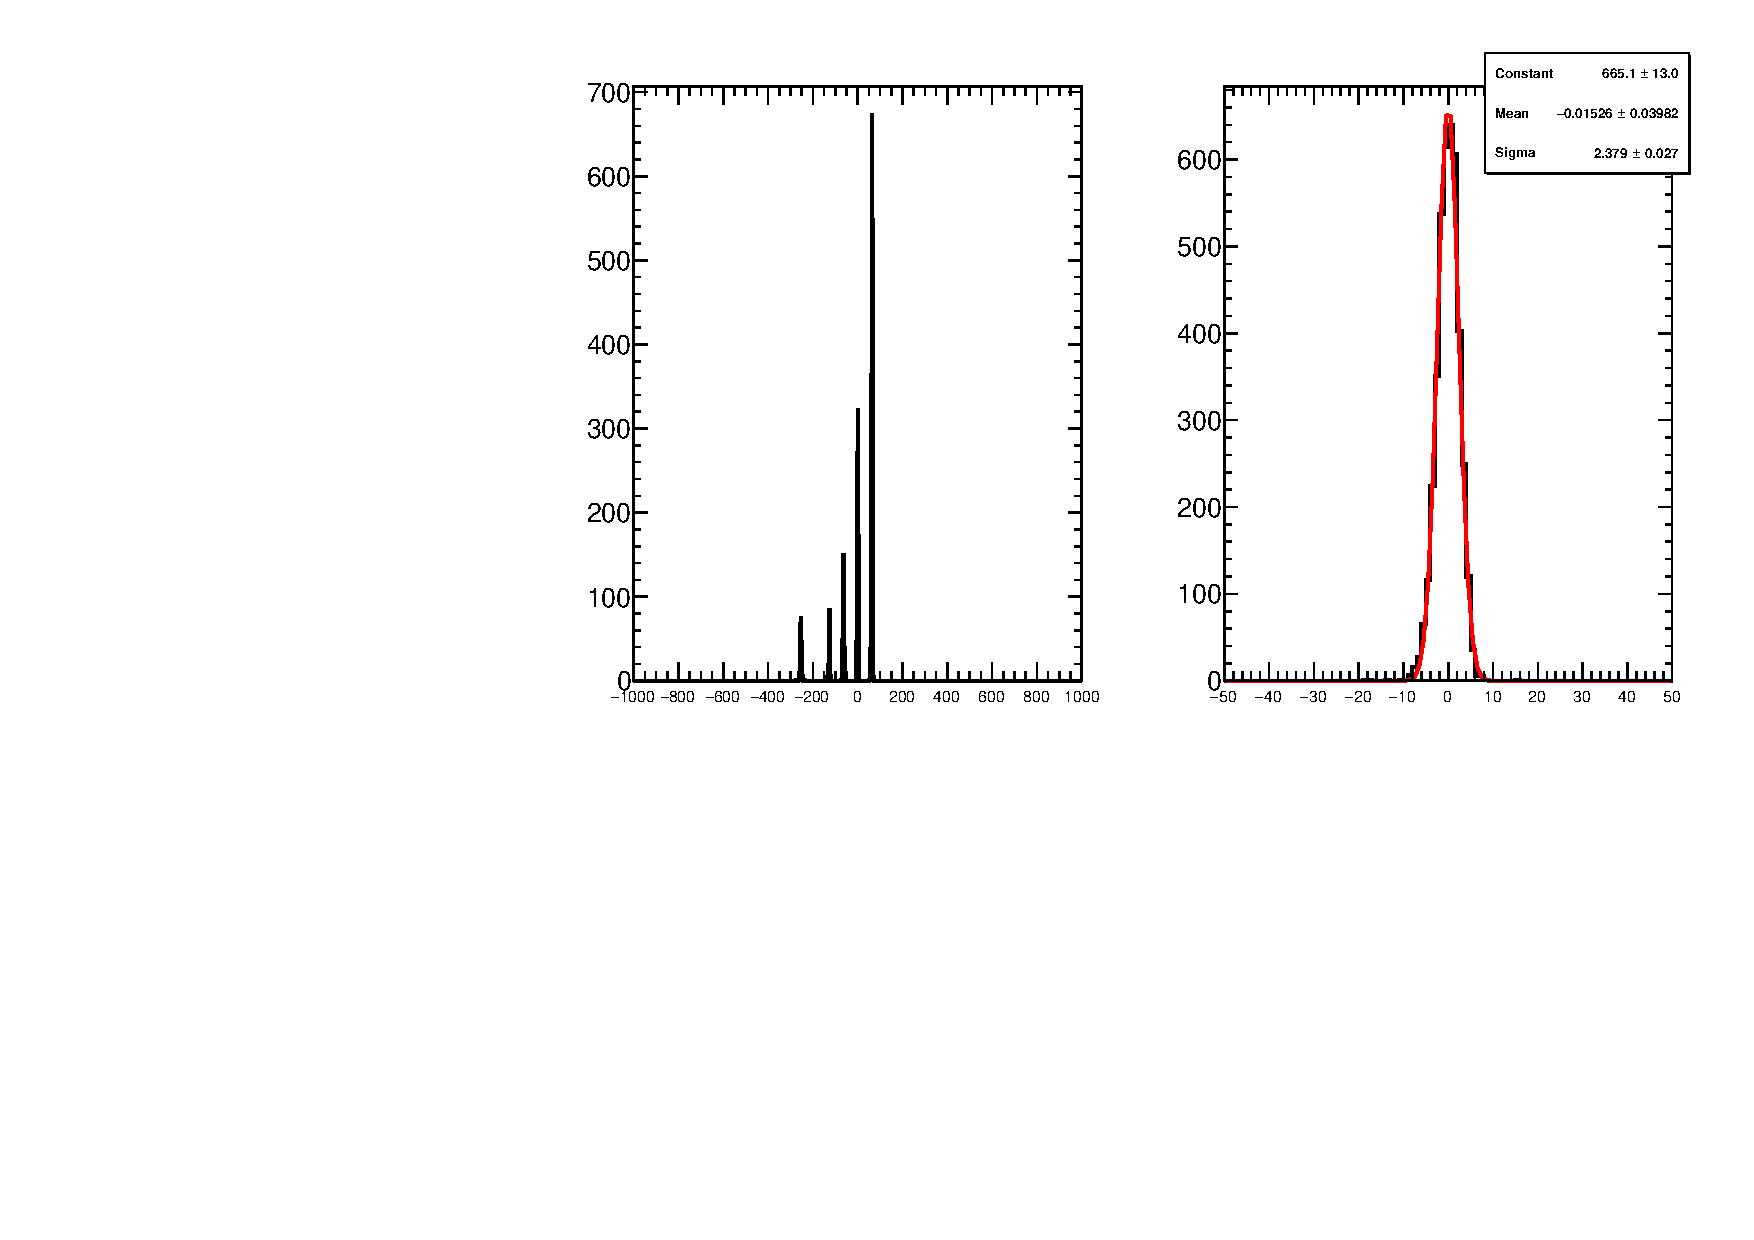
\includegraphics[width=0.9\textwidth]{images/(0,0).pdf}
\caption{Example of frequency calibrations for the FPGA Adjacent to the Zybo, $T_{cal} = 250~\unit{ms}$.
Shown is the reconstructed frequency for the base node FPGA at (0,0) within the QDB tile.
Figure~\ref{fig:fast_example} shows the corresponding reconstructed frequency pattern that represents the five individual peaks on the left.
A mean subtraction is performed on all five histograms to produce the right image, where a Gaussian fit is performed to estimate a frequency uncertainty ($\sigma$).
}
\label{fig:frq_recon_node00}
\end{figure}

\begin{figure}[]
\centering
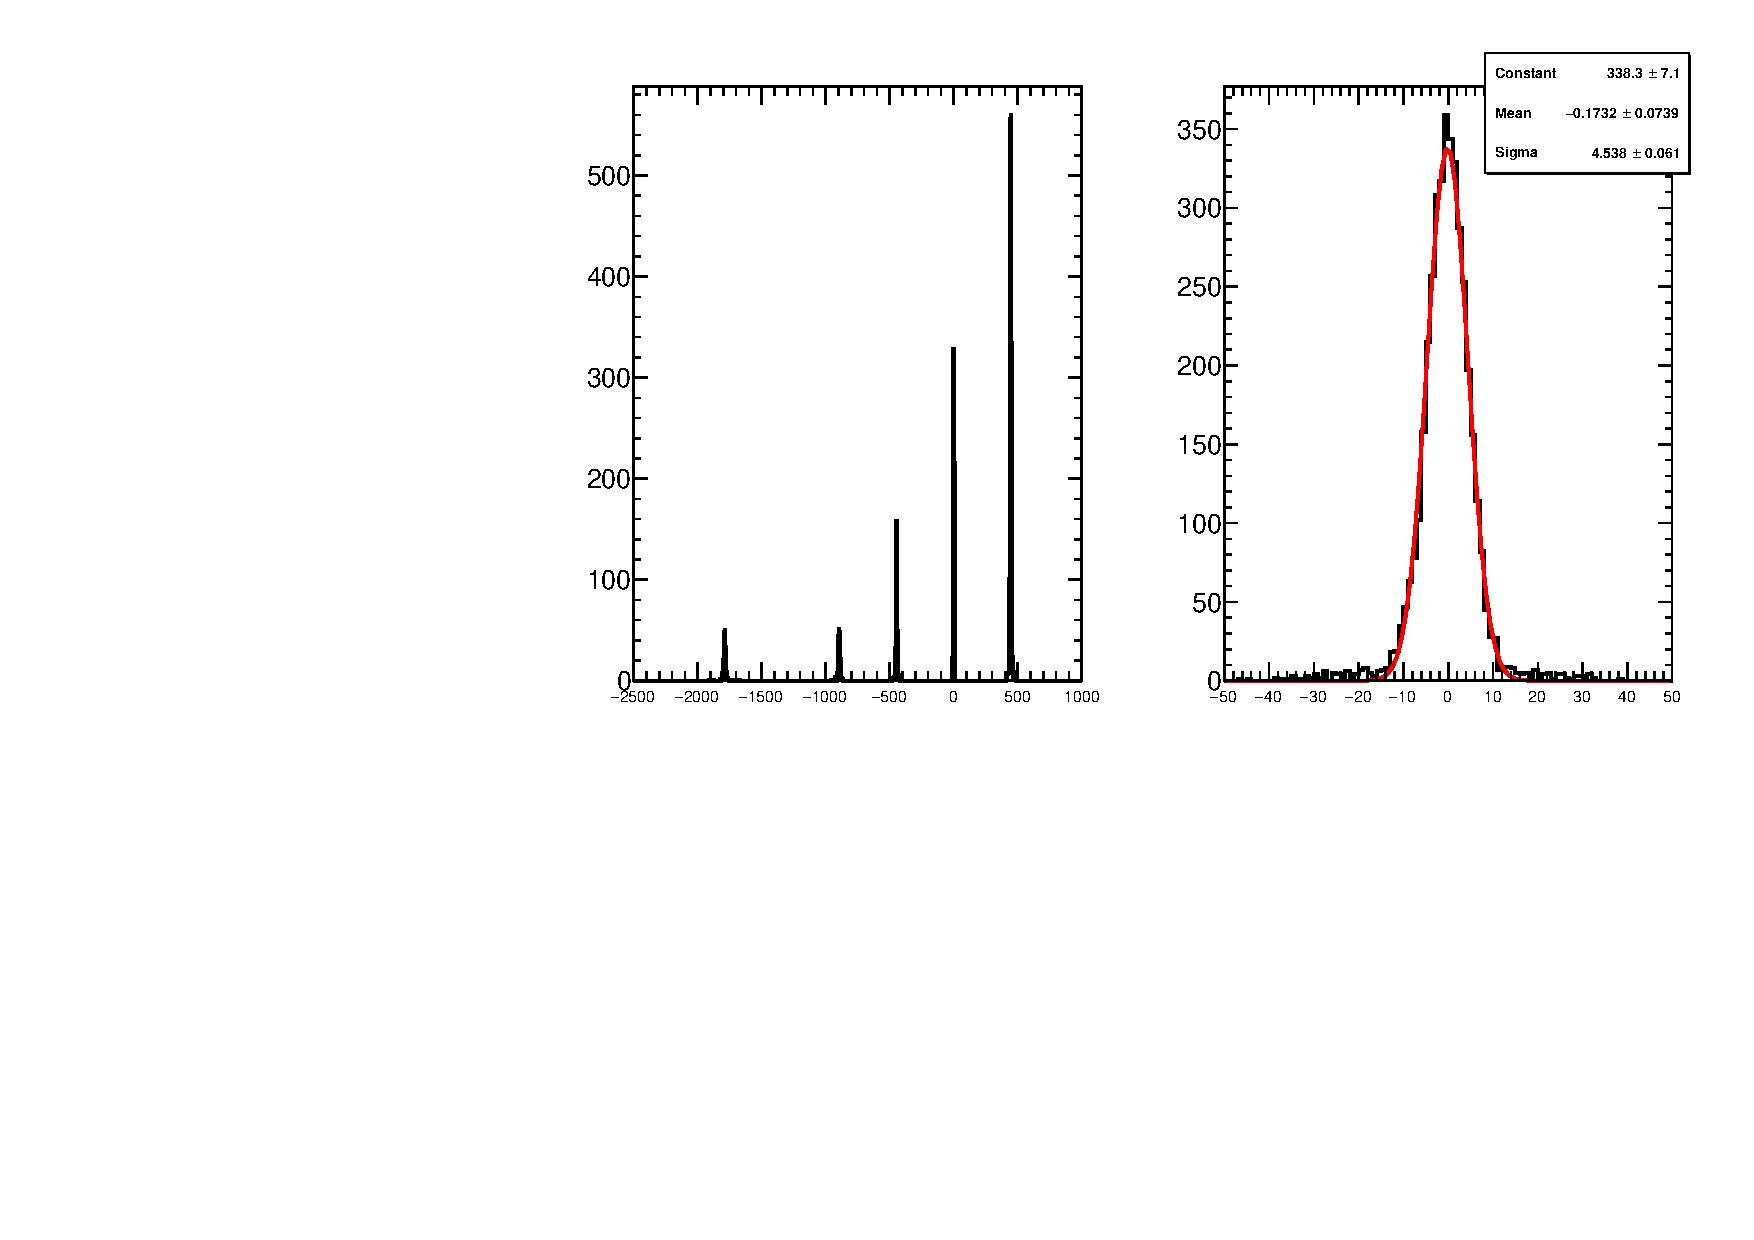
\includegraphics[width=0.9\textwidth]{images/(3,3).pdf}
\caption{Reconstructed frequency of the FPGA at position (3,3) within the QDB tile.
The relative drifts of the frequencies shown for the more distance FPGA are greater than the base node (0,0), which is only one transaction away from the aggregator.
}
\label{fig:frq_recon_node33}
\end{figure}


Figures~\ref{fig:frq_recon_node00} and~\ref{fig:frq_recon_node33} show that there are five distinct frequency groupings for the reconstruction.
These separate distribution of frequencies clearly correspond to the interrogation number of the Zybo as shown in Figure~\ref{fig:fast_example}.
The observed drift is inherent to that of the Zybo clock.
The reconstruction formula (Equation~\ref{eq:frequency_reconstruction}) on the frequency of the aggregator ($f_{a}$).
Therefore the uniform drift seen on all FPGAs can be attributed to the drift on the aggregator.

We remove this drift for each of the distributions by fitting a Gaussian to each of the distributions seen in Figure~\ref{fig:frq_recon_node33}.
Five Gaussian are fit to correspond to the five clusters, where the mean of the this fit are subtracted from the reconstructed points closed to this mean.
These news points form average frequency as shown in the right of Figures~\ref{fig:frq_recon_node33} and~\ref{fig:frq_recon_node00}.
A final Gaussian is fit where we use the $\sigma$ of the fit as the estimated uncertainty ($\delta f_{j}$) of each FPGA.
These results are shown for both the slow and fast interrogation frequencies in Tables~\ref{tab:fpga_calibration} and~\ref{tab:fpga_slow_calibration}.


\begin{figure}[]
\centering
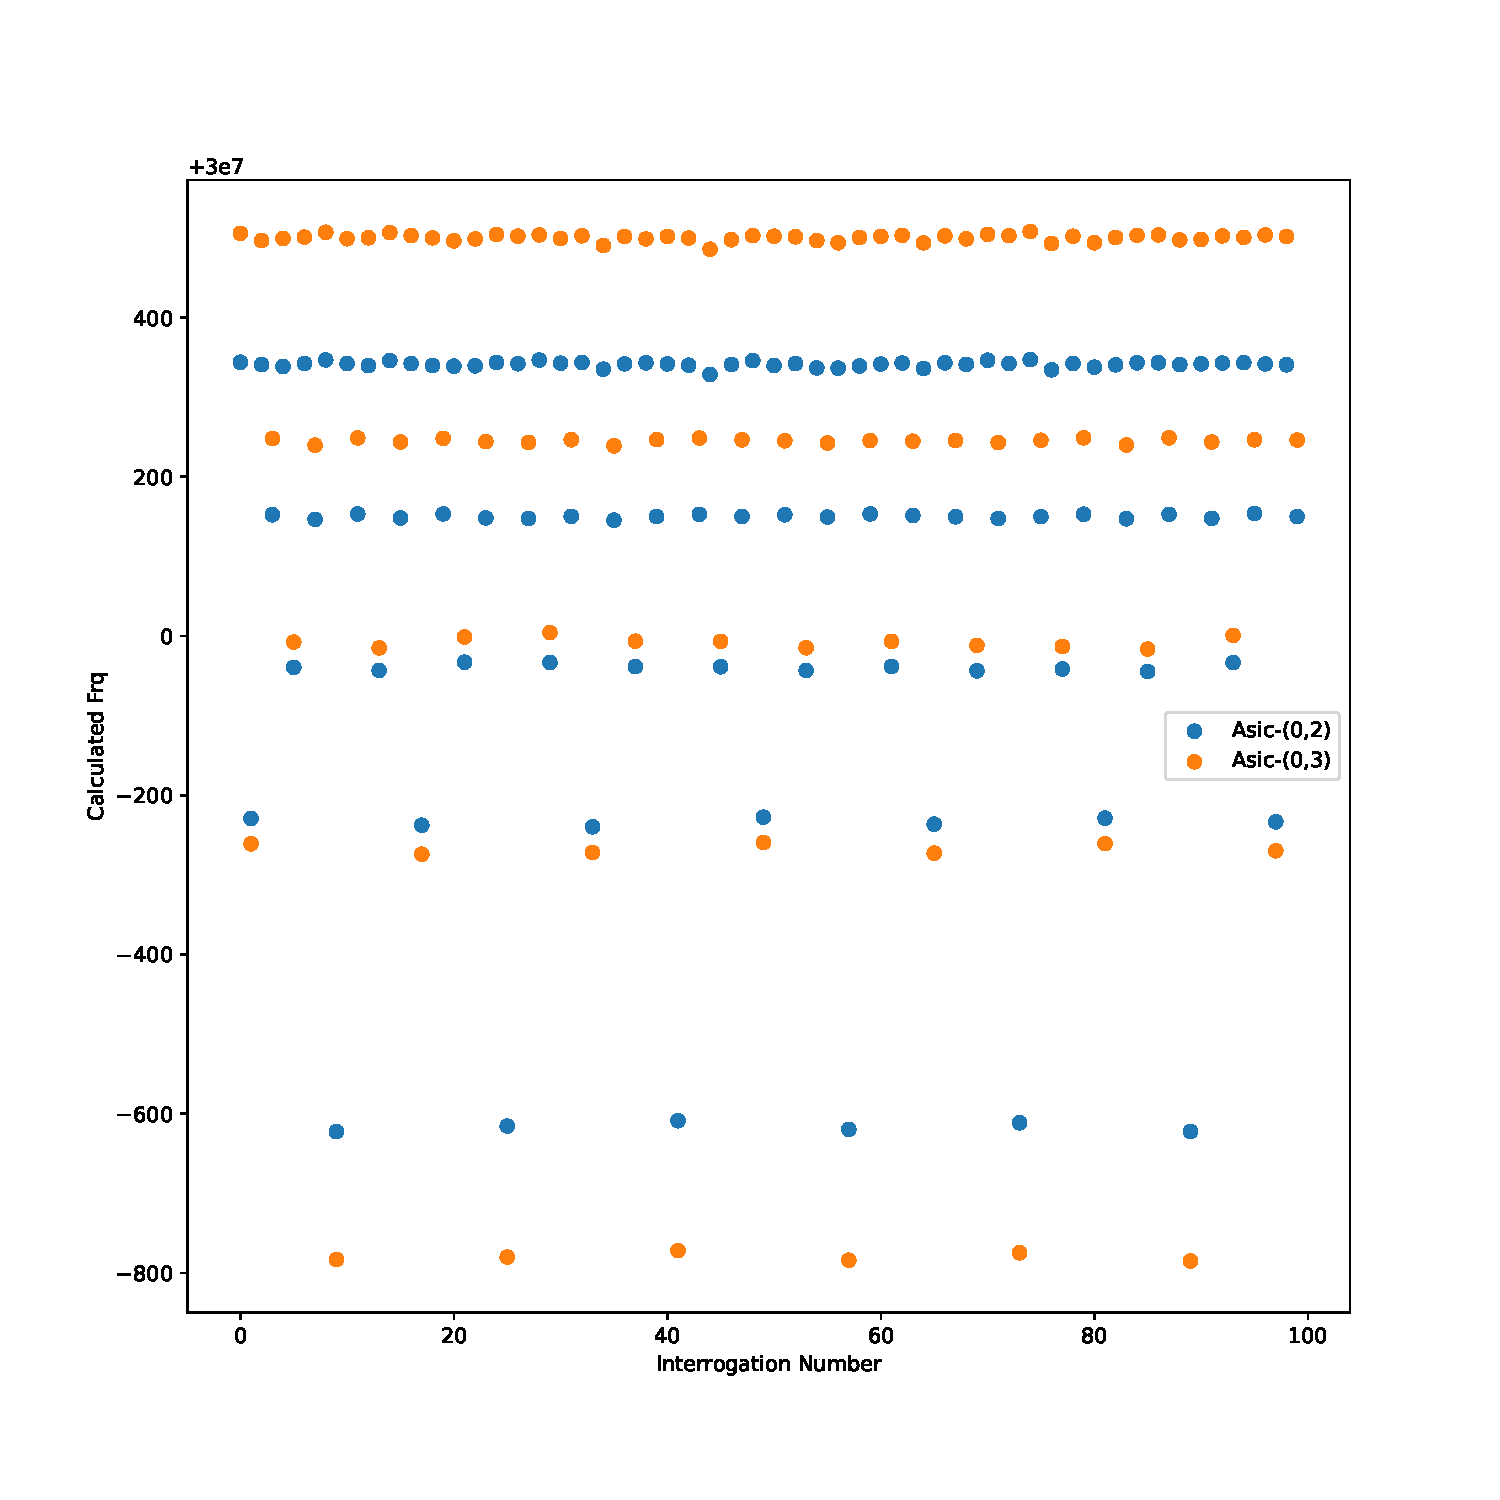
\includegraphics[width=0.9\textwidth]{images/fast_example.pdf}
\caption{Fast calibration procedure results for two different FPGAs.
Plotted are the reconstructed frequencies for increasing interrogation numbers.
Each interrogation is separated by approximately 250~\unit{ms}.
There is a repeating pattern of five distinguishable reconstructed frequencies plotted for two different FPGAs.
All 16 FPGAs follow this similar pattern, indicating that each of the reconstructed frequencies are varied by the aggregator's oscillator.
}
\label{fig:fast_example}
\end{figure}

\begin{figure}[]
\centering
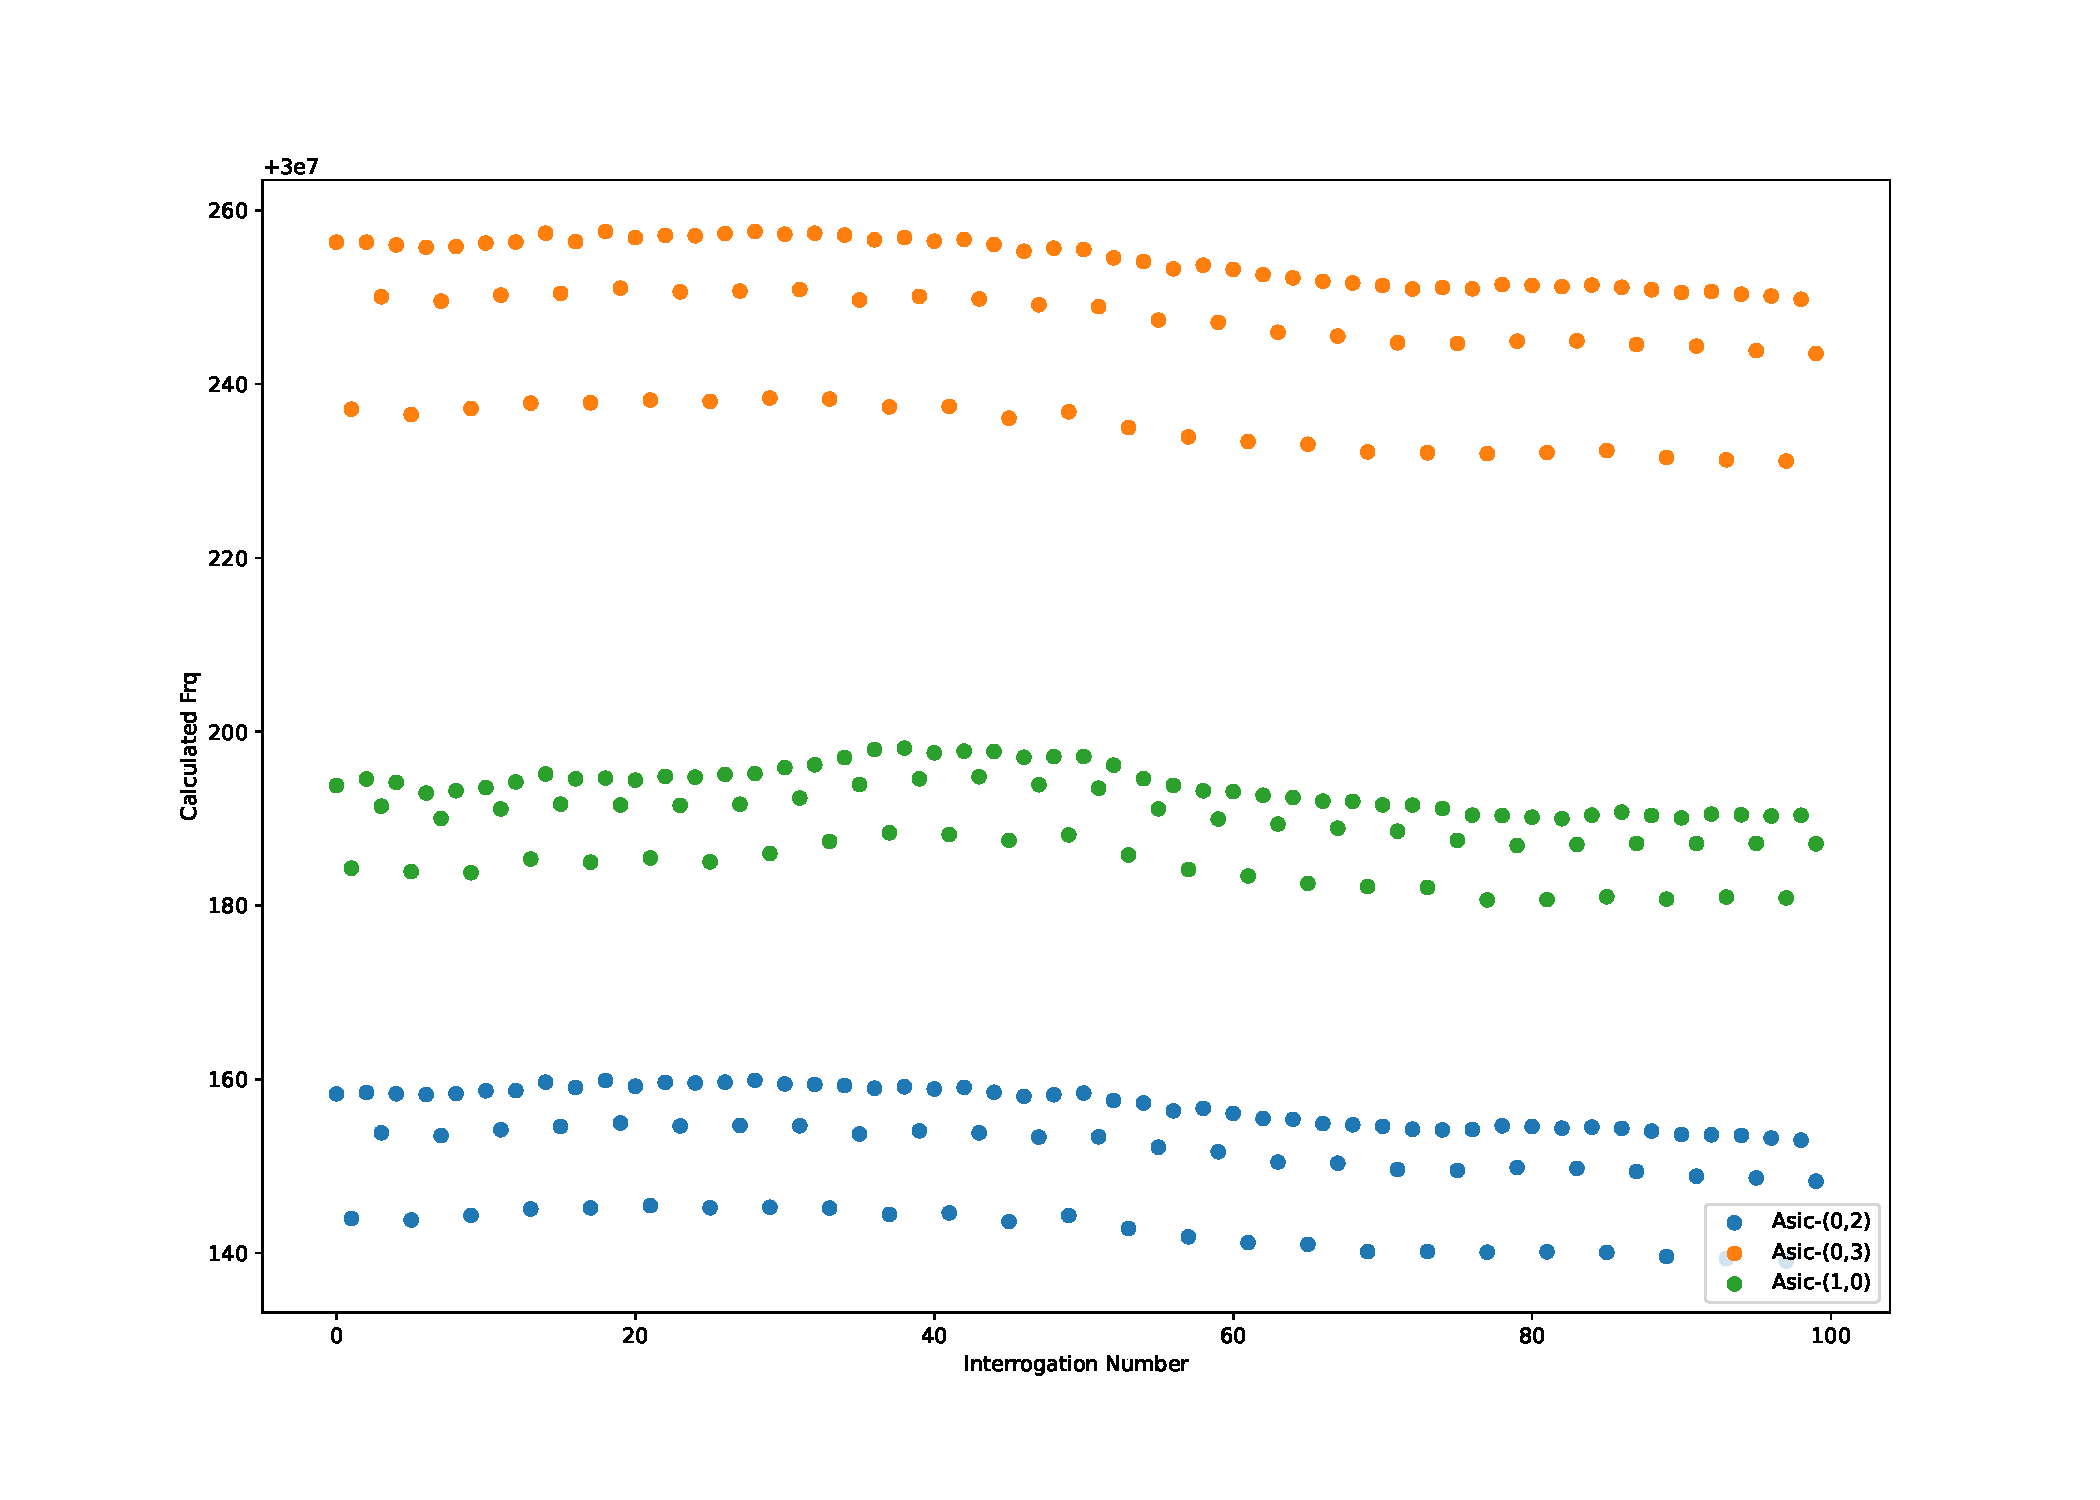
\includegraphics[width=0.9\textwidth]{images/slow_example.pdf}
\caption{Slow calibration example ($T_{cal} = 10~\unit{s}$).
A similar periodic behavior is seen in the slow calibration results as compared to the fast.
The drift of the three observable frequency drifts for the Zybo are clearly visible for the three FPGA frequency reconstructions shown. 
}
\end{figure}

%% 4Hz interrogation calibration 
\begin{table}
	\begin{center}
		\begin{tabular}{|c|c|c|c|}
			\hline
			FPGA Position & Mean (30~\unit{MHz}) & STD & $\frac{\delta f}{f_{o}}$*1e6 (ppm) \\
			\hline
			(0,0) & 245.543 & 2.379 & 0.079 \\
			\hline
			(0,1) & 190.646 & 2.979 & 0.099 \\
			\hline
			(0,2) & 153.908 & 3.334 & 0.111 \\
			\hline
			(0,3) & 248.831 & 3.843 & 0.128 \\
			\hline
			(1,0) & 192.729 & 2.860 & 0.095 \\
			\hline
			(1,1) & 210.905 & 3.405 & 0.114 \\
			\hline
			(1,2) & 116.212 & 3.984 & 0.133 \\
			\hline
			(1,3) & 159.824 & 4.158 & 0.139 \\
			\hline
			(2,0) & 351.431 & 3.685 & 0.123 \\
			\hline
			(2,1) & 193.845 & 4.285 & 0.143 \\
			\hline
			(2,2) & 200.278 & 4.071 & 0.136 \\
			\hline
			(2,3) & 152.633 & 4.263 & 0.142 \\
			\hline
			(3,0) & 183.359 & 3.954 & 0.132 \\
			\hline
			(3,1) & 209.788 & 4.561 & 0.152 \\
			\hline
			(3,2) & 192.277 & 4.169 & 0.139 \\
			\hline
			(3,3) & 171.302 & 4.538 & 0.151 \\
			\hline
		\end{tabular}
	\end{center}
	\caption{FPGA calibration results based on Hard Intterrogations at a frequnecy of 4~\unit{Hz}.
	The mean and standard deviation (STD) values are reconstructed for each ASIC within the tile as done in Figure~\ref{fig:frq_recon_node00} and ~\ref{fig:frq_recon_node33}.
	The listed STD value is the result of a gaussian fit performed on the adjusted frequencies.
	}
	\label{tab:fpga_calibration}
\end{table}


%% 0.1 Hz interrogation calibration 
\begin{table}
	\begin{center}
		\begin{tabular}{|c|c|c|c|}
			\hline
			FPGA Position & Mean (30~\unit{MHz}) & STD & $\frac{\delta f}{f_{o}}$*1e6 (ppm) \\
			\hline
			(0,0) & 243.223 & 3.895 & 0.130 \\
			\hline
			(0,1) & 187.225 & 4.631 & 0.154 \\
			\hline
			(0,2) & 151.020 & 6.255 & 0.208 \\
			\hline
			(0,3) & 246.553 & 8.229 & 0.274 \\
			\hline
			(1,0) & 188.851 & 4.521 & 0.151 \\
			\hline
			(1,1) & 207.837 & 6.468 & 0.216 \\
			\hline
			(1,2) & 111.344 & 7.882 & 0.263 \\
			\hline
			(1,3) & 156.660 & 9.985 & 0.333 \\
			\hline
			(2,0) & 348.263 & 6.748 & 0.225 \\
			\hline
			(2,1) & 190.976 & 8.622 & 0.287 \\
			\hline
			(2,2) & 196.369 & 9.919 & 0.331 \\
			\hline
			(2,3) & 148.284 & 11.844 & 0.395 \\
			\hline
			(3,0) & 179.718 & 8.375 & 0.279 \\
			\hline
			(3,1) & 207.859 & 10.655 & 0.355 \\
			\hline
			(3,2) & 188.123 & 11.836 & 0.395 \\
			\hline
			(3,3) & 165.011 & 13.725 & 0.457 \\
			\hline
		\end{tabular}
	\end{center}
	\caption{FPGA calibration results based on hard interrogations at a frequnecy of 0.1~\unit{Hz}.
	These data are more tightly clusted together due to the longer wait time between each interrogation, and are not easily separable as done in Table~\ref{tab:fpga_calibration}.
	The listed mean is the simple geometric mean and standard deviation for a one hour run time.
	}
	\label{tab:fpga_slow_calibration}
\end{table}

\subsection{Timing Stability and Communication Verification}
\label{sec:timing_test_results}
To estimate the reliability of the packet communication we calculate the number of total successful transactions.
During each hard interrogation each FPGA sends a broadcast register command plus the event end word as a response.
Then, for every hard interrogation there are at least 32 successful packet transactions. 
However, the routing used during the frequency calibration was snake routing, so the average traversal of each response packet (the number of FPGAs used to send each packet), is half of the array, plus one: 9.
Therefore, each interrogation required 16 correct broadcast packets plus $9\cdot 16 = 144$ successful response packets, for a total of 160 packets.
The total number of interrogations between both frequency tests was over 7000.
This corresponds to at least 1,120,000 successful packet transactions.

Also, performed was a sequence of random register writes followed by read requests perform on each FPGA to the channel mask register (See Table~\ref{table:node_registers}).
The channel mask register is a proxy scratch register, since it allows the reading and writing of any 16 bits.
We performed a long run ($\approx$ 10~\unit{hours}) where the Zybo would write to a random FPGA a random sequence of 16 bits, followed by a read.
An error check was be performed on any mismatch between the two bytes read and written.
This read and write sequence occurred every 0.25 seconds, or 4~\unit{Hz}, for a total of an expected 144,000 transactions.
Each test, on average, writes an FPGA which is four transactions from the aggregator, and requires 8 transactions to respond.
This requires 12 correct packets for each read and write, for a total of 24 correct packets per test.
This readout successful tested another $\approx 24\cdot 144,000 = 3,456,000$ packets.
In total, an estimated 4,576,000 variable packets have been successfully sent without a single packet loss on the QDBs.

\begin{figure}[]
\centering
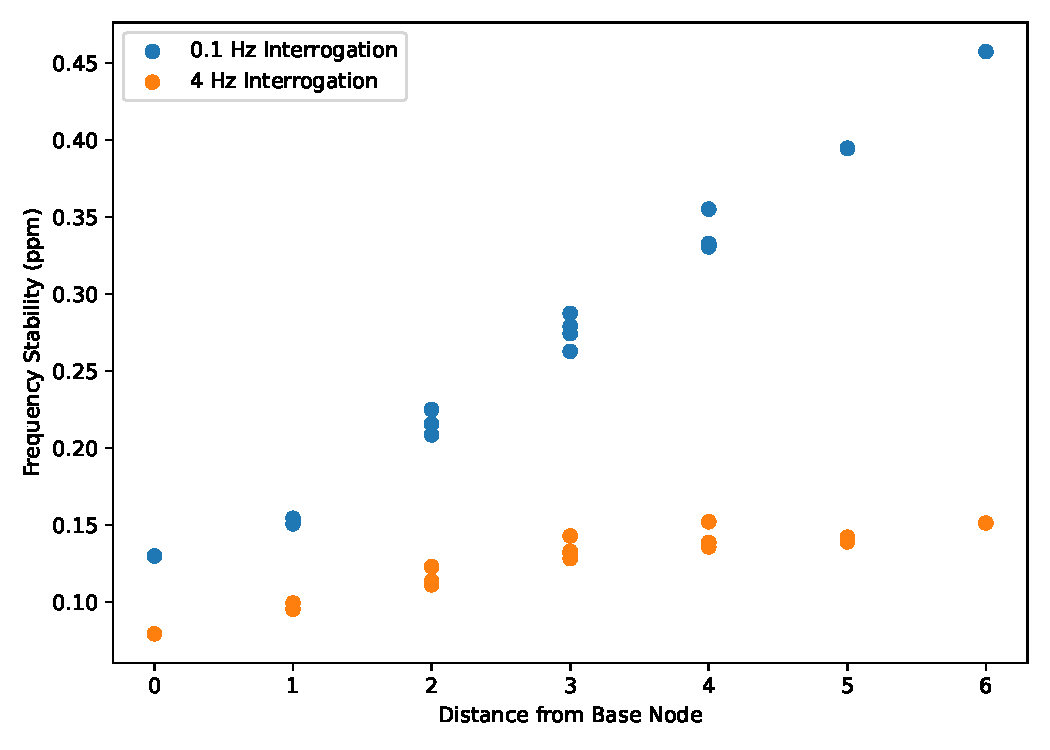
\includegraphics[width=0.8\textwidth]{images/interrogation_ppm_diff.pdf}
\caption{Shown are the relative values of the frequency part-per-million (ppm) values from the frequency calibration procedure in both the 4~\unit{Hz} (orange) and 0.1~\unit{Hz} tests.
The x-axis represents the number of transactions required to reach the FPGA.
These data are taken from Tables~\ref{tab:fpga_calibration} and~\ref{tab:fpga_slow_calibration}.
Clearly indicated is the relationship between the interrogation rate: a faster interrogation leads to a sharper average time reconstruction.
Also shown is that the further each FPGA is from the base node, the worse the frequency reconstruction is.
This happens since there are more average clock cycles to reach the remote ASIC (see Equation~\ref{eq:calib_constraints}).
}
\label{fig:calibration_position}
\end{figure}

Figure~\ref{fig:calibration_position} relates the calculated frequency stability of the QDB tile using the slow and fast calibration modes.
The results show that the slow calibration mode produces a higher frequency ppm than the fast interrogation method. 
This indicates that the rate of the interrogation in the final system can be used to compensate for a less stable oscillator at ASICs further from the base node.
Also shown is that for both interrogation rates is that the result of the reconstruction depends on the FPGA (ASIC) location within a tile.
These results (with the ASIC oscillator frequencies) indicate a limit to how large a tile can constructed.
The distance from the base node indicates the number of packet transactions that the interrogation must proceed through the tile before the Event End word is constructed.
This means that fully connected tiles (FCT) will allow for largest tiles with local oscillators, since they provide the shortest path from the base node to any remote node.

\section{The Digital Back-End Summary}
The Q-Pix digital back-end is expressed as a collection of inter-connected nodes as presented in Section~\ref{sec:digital_constraints}.
Each node represents an ASIC which connects to the front-end, which for Q-Pix is a collection of integrating CSA for each pixel in the TPC.
The Q-Pix ASIC design is presented in Section~\ref{sec:digital_prototype}, where we define its response to inputs by its FSM in Section~\ref{sec:digital_fsm}

The full Q-Pix readout is handles the large number of connections required in a DUNE-FD ($\simeq 58,000$ per APA) by first collecting data via an aggregator node.
The QDB prototype (described in Section~\ref{sec:qdb_prototype}) implements this first use of a Q-Pix tile and aggregator system.
The use of a controllable aggregator removes the the need for ASICs to dynamically self configure, and dramatically reduces the number of connections to collect all data.
Each ASIC allows a configurable routing direction which is controlled by packets created at the aggregator.

The basic unit of the Q-Pix DAQ can be thought of as a tile and aggregator system, where one or more tiles are assigned to a single aggregator.
Future implementations of Q-Pix can readily assign multiple tiles per aggregator.
The number of tiles that an aggregator can be assigned to is dependent on its available pins as well as its maximum data output.
Each aggregator will require at least two pairs of differential pins to connect to abase node per tile, as well as provide at least $117~\unit{kB}$ of data output either to disc or another controlling node per connected tile.

The results of the QDBs~(Section~\ref{sec:qdb_prototype}) demonstrate the reliability of the communication protocol to more than 1 million packets.
The calibration procedure is able to reconstruct remote FPGA frequencies in a Q-Pix 4$\times$4 tile to better than 1 ppm ($\frac{\delta f_{o}}{f_{o}}$).
We also find that the size of a tile is limited by the oscillator frequencies of the ASICs as well as the aggregator.

In Chapter~\ref{chap:sim} we explore simulations of the Q-Pix tile system and explore its ability to analyze radiogenic backgrounds and capture beam neutrino events.
